\chapter{Traffic engineering in content-dominated networks}
\label{ch:te-background}

This chapter serves two main purposes. First, is to provide the reader with necessary background on traffic engineering in ISPs, content delivery and prior work on the interaction between traffic engineering and content delivery. Second, is to explain the motivation for our work on traffic engineering in content-dominated networks in light of the existing work in this area.

To that end, this section has the following key objectives:
\begin{itemize}
	\item
	explain the common traffic engineering approaches and cost objectives in the context of an Internet service provider
	\item
	explain the content delivery techniques used by Content Deilvery Networks (CDNs) towards improving user-perceived performance.
	\item
	review prior literature on the interaction between traffic engineering and content delivery, in particular the interaction between overlay routing and network routing, and request redirection and network routing.
	\item
	make a case for studying the interaction between content placement and network routing by illustrating this interaction using examples. 
\end{itemize}


%Traffic engineering done by Internet service providers focuses on  computing the routing in the network for optimizing cost and other objectives. But, traffic engineering techniques are not isolated from mechanisms that alter the flow of traffic from the application. In particular, decisions at the application-layer ``overlay networks'' such as content placement and redirection also seek to alter how traffic flows in the network. Motivated by this observation, a question of long standing interest has been the following: 

%\emph{what influence do the decisions at the overlay have on the routing strategies of the underlying network, and vice versa?} 



%Internet is composed of independently controlled sub-networks called autonomous systems. an isp is one such autonomous system. an isp does traffic engineering to configure routing. in a content-dominated network, application-level decisions on content placement and request redirection affect traffic engineering. the high goal of this part of this thesis is to design and to evaluate traffic engineering schemes while accounting for the interaction with content delivery decisions. the focus on evaluating the role of content placement  while studying this interaction distinguishes us from prior work in this area.

%This chapter provides background on content delivery and traffic engineering and makes a case for studying the role of content placement on this interaction. Chapter x and Chapter y studies traffic engineering in two scenarios with varying degrees of flexiblity in placing content. Chapter x focuses on an ISP network in a fixed content placement policy, namely that of placing content at multiple locations chosen randomly. While, Chapter y focuses on a network CDN, an ISP that deploys a CDN to deliver content to users on its network and enjoys full freedom to control the placement and routing on its network. 

\section{Traffic engineering}

The goal of traffic engineering (TE)  is to avoid congestion hotspots in the network by optimizing routes based on network topology and expected traffic demand. In the context of large Internet service provider (ISP) networks, traffic engineering decides both intra-domain (within the ISP) and inter-domain routing (across ISPs). We focus here on intra-domain routing and refer the reader to  \cite{Feamster2003,rexford} for a survey of inter-domain traffic engineering. 


Traffic engineering schemes are commonly evaluated based on cost functions that are a function of utilization of network links. Link utilization is a relevant metric because a low utilization of all links implies that the network is free from congestion hotspots and has spare capacity to tolerate an increase in demand. A well-known cost function is maximum link utilization or MLU. We give a simple example to show how traffic engineering can reduce link utilization.


If the traffic matrix is known accurately, the optimal solution to the traffic engineering problem can formulated as a multi-commodity flow optimization problem. The routing thus computed is reffered to as \emph{Optimal TE} in literature. But, it is impossible to have accurately knowledge of future traffic matrices. Therefore, practical traffic engineering schemes either take a demand-aware or a demand-oblivious approach.  A demand-aware TE periodically updates routing using historically observed traffic matrices. A demand-oblivious TE requires no explicit measurement of traffic matices, but instead configures routing statically. A demand-oblivious TE is simpler to implement because it requires neither measuremnt nor periodic updating of network routing. But, demand-aware schemes have been shown to outperform demand-oblivious TE.

In practice, offline TE based on Open Shortest Path First (OSPF) and Multiprotocol Label Switching (MPLS) are commonly used  \cite{COPE,MultiTM,fortz2000internet,MPLS2}. Routes computed by OSPF traffic engineering must follow shortest-weight paths, therefore OSPF TE provides limited functionality to split traffic among multiple paths. MPLS TE overcomes this limitation by enabling traffic between two nodes to be split  in arbitrary ratios among multiple paths. Therefore, MPLS TE gives better results than OSPF TE as exemplified by the above example \cite{COPE,MultiTM}.

%Therefore, TE schemes commonly take a demand-aware approach, i.e., they compute routing using historically observed traffic matrices. In contrast, demand-oblivious simpler schemes also exist, no measurement of traffic matrix or continual updating of configuration. 

%But, future demand is not known perfectly. So, TE schemes commonly take a demand-aware approach: use historic demand patterns to predict future demand. In contrast, demand-oblivious simpler schemes also exist, no measurement of traffic matrix or continual updating of configuration. Demand-oblivious is simpler but demand-aware schemes have been shown to outperform them in TE literatue.

%
%Cost-based metrics: ignored the impact on end-user performance. So, what is the impact on end-user performance.
%
%TE is isolation, ignoring the internation with content placement and redirection.
%
%How do TE schemes compare when accounting for the interaction with content delivery.



\section{Content delivery}

Content delivery systems seek to provide a high-quality experience to users accessing content in all regions  at all times. A canonical example of a content delivery system is a content delivery network (CDN). State-of-the-art CDNs operate geo-distributed datacenters, and use a combination of edge caching, intelligent server selection, and path and protocol optimizations for delivery of several types of content, e.g., video, bulk downloads, and interactive websites \cite{DilleyMPPSW02,akamai-overview}. Given their geo-distributed deployment, the decisions of content placement, i.e., locations at which a content is placed, and request redirection, i.e., which location is best positioned to serve a user's request, are central to the functioning of a CDN.

\textbf{Content placement:} Content placement in CDNs is commonly done using caching schemes. For example a commonly used caching strategy is least recently used (LRU) cache replacement. There are two reason why content cahing is widely used. First, caching naturally captures geographic and temporal locality in content requests to populate caches with content likely to be reused. Second, a vast majority of network traffic is generated by content that gets updated infrequently, e.g., a video, audio, images. As a result, cached copies of content remain reusable for long duration. 



Strong consistency is a separate topic and is studied in the content of design of geo-distrbuted kv store in auspice.\tbd{fix this}

\textbf{Request redirection:} Request redirection strategies complement placement strategies by selecting the server location that is best suited to process a user's request. These strategies have been extensively studied and form the heart of CDN technology today. To quote from a report by Akamai,  \emph{``the system directs client requests to the nearest available server likely to have the requested content."} where the ``nearest" server is one whose round trip latency as well as packet losses are small, and  an ``available" server is one that is lightly loaded considering all resources, i.e., network, CPU and disk  \cite{DilleyMPPSW02}. 

Request redirection is implemented using three processes: (1) \emph{Monitoring:} Probe messages sent intermittently help monitor network characteristics and server load and identify congested regions of network and overloaded server locations \cite{oasis,donar}. (2) \emph{Estimating distances:} The measured statistics are combined to compute a distance function that reflects the proximity of a server location to users in a geographic region \cite{donar}. (3) \emph{Informing the user:} The user is informed of selected server/s either via DNS resolution or via HTTP redirection as described in  \cite{DilleyMPPSW02} and  \cite{barbir2003known}.


Drawing parallels between our classification of traffic engineering schemes into demand-oblivious and demand-aware, we consider common content delivery techniques discussed above to be demand-oblivious since they do not require explicit measurement of content demand. In contrast, a demand-aware approach to content placement and redirection has been studied in research also, e.g., Applegate \emph{et al.} use a demand-aware approach to determine placement and redirection for Video-on-Demand content in the network. 


\section{Interaction between traffic engineering and content delivery}

Content delivery routes traffic at the application layer using an overlay network of servers, and traffic enginering configures network routing of the underlying physical paths. Studying this interaction between decisions at the overlay and the underlying network has a topic of long standing interest in computer science. Several related questions have been put forth. Does the interaction between network routing and content delivery yield sub-optimal results? How can we design cooperative mechanisms to leverage these interactions? Do cooperative mechanisms yield benefit in an Internet-like environment? We find that nearly all previous research on this topic has focused either on the interaction of overlay routing with the network routing \cite{Roughgarden,selfishQiu}, or that of server selection strategies with the underlying routing  \cite{Jiang2009,JohariGameTheory, CATE, P4P} as discussed below. 


%Studying the interaction between network and content delivery has been a topic of much interest in both systems and theory communities. Several related questions have been put forth. Do these interactions negatively affect objectives of networks and content delivery systems? What is the sub-optimality caused due to these interactions in the worst case, and for typical topologies and traffic demands? How to leverage these interactions to improve traffic engineering and content delivery objectives? 

%Yet, we don't fully understand these interactions because prior research has studied the interaction of network routing with only a subset of content delivery decisions. Much prior research has focused on two aspects: the interaction of overlay routing and network routing  \cite{Roughgarden,selfishQiu}, and the interaction of request redirection and network routing  \cite{Jiang2009,JohariGameTheory, CATE, P4P}. While placement decisions are critical to user-perceived performance, there has been little research on how content placement interacts with network routing.

\textbf{Interaction between traffic engineering and overlay routing:} Several results show the negative interaction between selfish overlay routing and network routing \cite{Roughgarden,selfishQiu}. Theoretical results indicate that the negative interaction could cause an arbitrary degradation in user perceived delay. Further studies using synthetic traffic demands and topologies indicate that this interaction hurt traffic engineering metrics. However, it appears that a small fraction of Internet traffic uses overlay routing.  For example, traffic from CDN edge server to the client always follows network routing. Further, overlay routing yields ``marginal" benefits ($<$ 30\%) over network routing for 79\%-96\% of paths depending on which geographic region is being considered  \cite{rahul2006overlays}, which suggests that traffic between CDN servers forming an overlay network follows network routing in most cases. For this reason, this thesis does not model the interaction between overlay and network routing.


\textbf{Interaction between traffic engineering and request redirection:} Recent research has investigated the interaction between request redirection and traffic engineering, without considering the role of placement strategies. This interaction is commonly studied in the context of Internet service providers (ISPs) and content providers (CPs) with geo-distributed datacenters. 
Both analytical results \cite{Jiang2009,JohariGameTheory} and system implementations \cite{CATE,P4P} have shown that there is value for joint optimization of request redirection and traffic engineering, and cooperative strategies can help traffic engineering metrics and also reduce user-perceived latencies. Commonly, these efforts assume that all content is available at all locations, ignoring the fact that content availability at a location depend on placement strategies. Therefore, in this thesis, we account for the effect of content placement along with request redirection, in studying the interaction between network and content delivery.


\section{Illustrating the interaction between content placement and traffic engineering}

We make a case for studying the interaction between content placement and traffic engineering by illustrating that content placement can change the traffic matrix. The first example shows that if content is placed at multiple fixed locations in the network, then merely updating network routes can change the traffic matrix. The second example shows that if content placement can be changed, it can change the traffic matrix in way that reduces network cost and enables simpler routing in the network.




\begin{figure}[tbh]
	\begin{center}
\label{fig:3node-bg}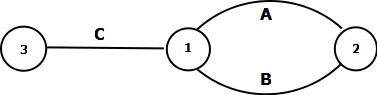
\includegraphics[scale=0.5]{final_images/Diagram3node.png}

	\caption{Lasso network}
	\end{center} 
	\end{figure}




%\textbf{explain conditions}
\textbf{Example 1:} In Figure~\ref{fig:3node-bg}, all links are assumed to have a capacity of 100 units and a constant delay. The top link A has a very small delay compared to the other two links that both have equal delay. Node 1 has 100 Mbps of demand that it can obtain from 2 as well as 3. In addition, there is 20 Mbps of demand at node 1 which it can obtain only from 2.  We assume that the aggregate demand at a node consists of a large number of user-initiated connections. When content can be downloaded from multiple locations, users initiate parallel TCP connections and the throughputs along paths in a parallel TCP connection are inversely proportional to the path delays. The TE scheme is assumed to be OSPF-based, i.e., shortest-path routing using configured link weights and traffic split equally among multiple paths with equal weights.

%\textbf{point: TE cannot be achieved since adaptation changes TM.}

Suppose the weights of the links A and B are unequal and the link A has more weight. As a result, all of the traffic between 1 and 2 is routed using only link B. 1 splits its demand of 100 Mbps using parallel TCP equally between links B and C. Thus, the traffic on links A, B, and C is  0, 70, and 50 respectively. In the next step, seeking to balance load better for this resultant matrix, the TE scheme sets both the links A and B to the same weight (hoping to achieve link utilizations of 35, 35, and 50 respectively).  Consider how parallel TCP connections respond to this change.
Assuming each TCP connection between 1--2 is pinned to only one of the two paths---as is commonly done in practice to achieve equal-cost multi-path (ECMP) splitting---50 Mbps of demand at 1 gets routed using parallel TCP connections over the link A and link C, and an equal amount using parallel TCP connections along the link B and link C. In addition, the 20 Mbps of background traffic is split equally among link A and link B as per ECMP.  Since link A has a much smaller delay than link C, the 50 Mbps of demand at 1 using parallel TCP along those two paths will flow entirely through link A. The remaining 50 Mbps using B and link C will get split equally across the two paths by parallel TCP. Thus, the traffic on the links A, B and C is 60, 35, and 25 respectively, which is different from what the TE scheme engineered for (namely, 35, 35, and 50). The resulting MLU of 0.6 is different compared to 0.5, the value that the TE scheme expected. 


\textbf{Example 2:}To appreciate how placement can shape traffic, consider the simple example in Figure~\ref{fig:NetworkExample}. Node $C$ has an object in its cache that is requested by end-users at nodes $A$ and $D$. Suppose that one unit of traffic needs to be routed from $C$ to $A$ and $0.5$ units  from $C$ to $D$ to satisfy the demand for that object. The routing that achieves the minimum MLU of $0.5$ to serve the demanded object is shown in the figure. Note that the routing that achieves the MLU of 0.5 is not possible with a simple, \unplanned\ protocol like InverseCap as that would route all the traffic demand from $C$ to $A$ via $B$, resulting in an MLU of 1. Thus, a (\planned) traffic engineering scheme is necessary to achieve an MLU of 0.5.


	\begin{figure}[h]
		\centering
		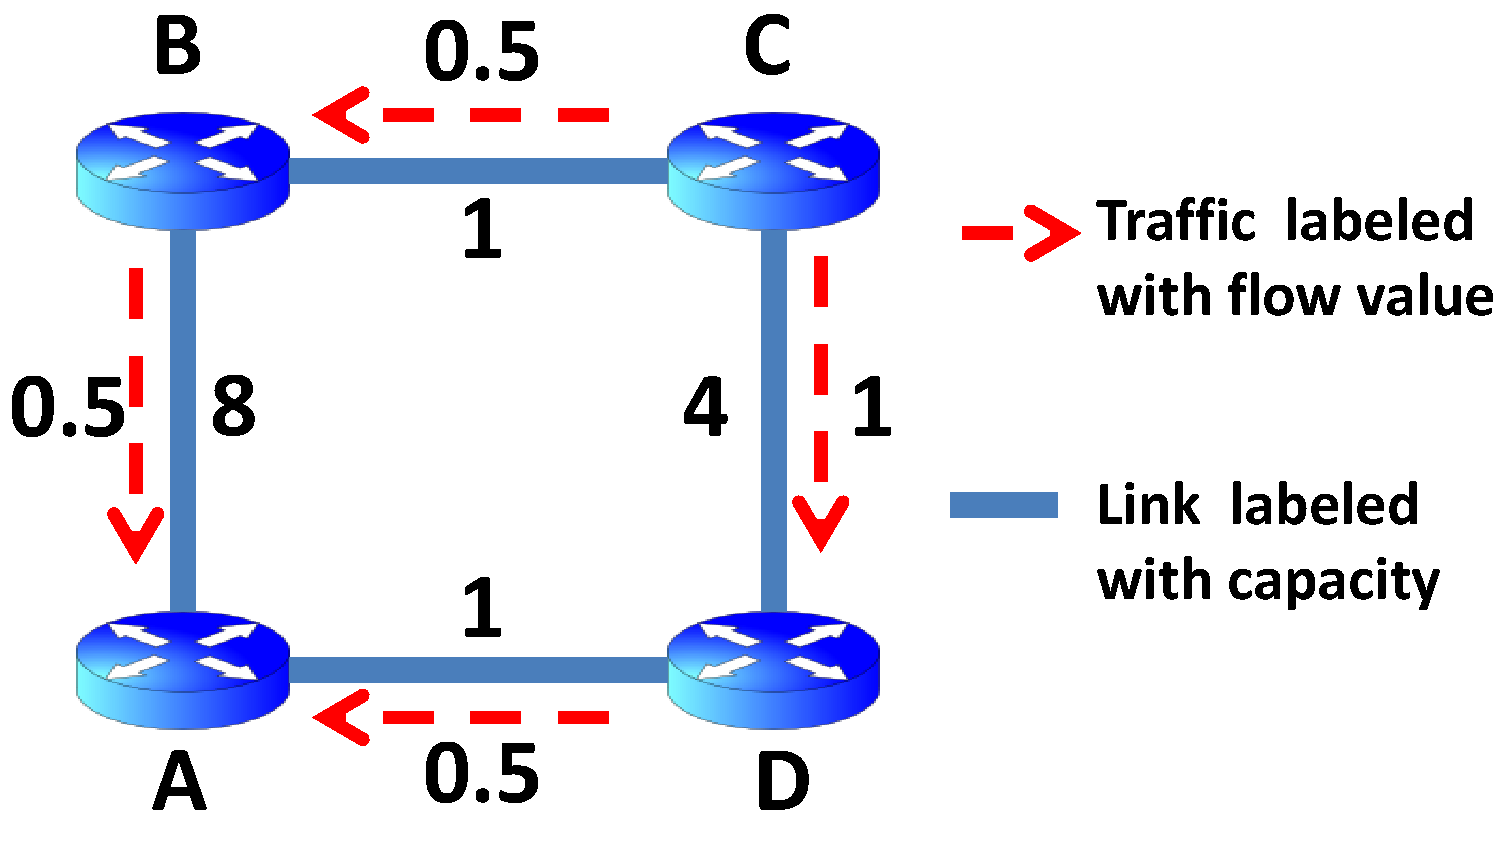
\includegraphics[width=2in]{ncdnpaper/ncdn-example}
		\caption{A Simple \ncp\ Example}
		\vspace{-.3in}
		\label{fig:NetworkExample}
	\end{figure}


On the other hand, NCDNs can shape the traffic demand matrix by using a judicious placement and redirection strategy. Suppose that there is some space left in the content server's cache at node $B$ to accommodate an additional copy of the demanded object. By creating an additional copy of the object at $B$, the traffic demand of $A$ can be satisfied from $B$ and the demand of $D$ from $C$ achieving an MLU of $0.125$. In this case, judicious content placement decreased the MLU by a factor of $4$. Even more interestingly, this best MLU can be achieved using a simple routing scheme like InverseCap while also improving user-perceived latency (assuming that the latency of link $BA$ is lower than that of the two-hop paths from $C$ to $A$).

\section{Research questions}

The above examples make a case for modeling the effect of content placement while studying the interaction between traffic engineeering and content delivery. Consequently, our work accounts for the interaction between placement, redirection and routing while addressing the following key questions: 

(1) How do well-known classes of traffic engineering schemes compare in terms of available capacity and end-user performance metrics?

(2) What is the relative importance of placement and routing for optimizng performance and cost objectives?

(3) If a network can control content delivery as well underlying routing, should that network follow simple demand-oblivious schemes for content placement and routing, or a more sophisticated scheme that jointly optimize these two decisions?


